\documentclass[conference]{IEEEtran}
\usepackage[utf8]{inputenc}
\usepackage[english,spanish]{babel}
\usepackage[T1]{fontenc}
%\usepackage[latin1]{inputenc}
\usepackage[utf8]{inputenc} 
\usepackage{indentfirst}
\setlength{\parindent}{8mm}
\usepackage{kantlipsum}
\usepackage{graphicx}
\usepackage{lipsum}

\newcommand\tab[1][1cm]{\hspace*{#1}}

\usepackage{hyperref}

\usepackage{subcaption}

\usepackage{booktabs,multirow,rotating}
\usepackage{tikz}
\usetikzlibrary{patterns,fit,backgrounds,arrows,calc} %,shapes,decorations.pathreplacing

\usepackage[
backend=biber,
style=trad-plain,%numeric-comp,%trad-plain,%apa,%review style bibstyle citestyle $3.3
natbib=true,%natbib compatibility $3.8.9
sorting=none,%sorting style nyt, nty
%maxnames=3, minnames=1,
%smartand=1,%y/e
maxbibnames=8, maxcitenames=3]{biblatex}
\DefineBibliographyStrings{spanish}{andothers={et~al\adddot}}

\addbibresource{bibliografia.bib}

\title{
 Desarrollo del Videojuego de Ajedrez con Programación Orientada a Objetos en C++\\ 
 }

\author{\IEEEauthorblockN{Carlos Mestas}
\IEEEauthorblockA{Escuela Profesional de Ingeniería \\de Sistemas\\
Universidad Nacional de San Agustín\\
Arequipa, Perú\\
cmestas@unsa.edu.pe}
\and
\IEEEauthorblockN{Lenin Usca}
\IEEEauthorblockA{Escuela Profesional de Ingeniería \\de Sistemas\\
Universidad Nacional de San Agustín\\
Arequipa, Perú\\
lusca@unsa.edu.pe}
\and
\IEEEauthorblockN{Oscar Cuadros}
\IEEEauthorblockA{Instituto de Ciências Matemáticas \\e de Computação, ICMC-USP\\
Sao Paulo, Brasil\\
ocuadrosl@unsa.edu.pe}}

\begin{document}
\maketitle

\renewcommand{\abstractname}{Resumen}
\begin{abstract}

El ajedrez es un juego milenario de estrategia, donde participan dos jugadores, cada uno de ellos controla un equipo de fichas, cada una con características distintas, donde el objetivo principal es capturar la ficha más importante de cada jugador, el Rey, al momento de que el Rey es capturado el juego termina. También tenemos la programación orientada a objetos que busca tener una mejor calidad de software con eficiencia y eficacia, viendo del punto de vista de la programación podemos tomar cada una de las fichas como un objeto y con atributos y características similares y diferentes. En el presente trabajo desarrollamos un juego en el lenguaje de programación C++ un videojuego de ajedrez, tomando en sí las características principales de este juego, movimiento de las fichas y funciones que tienen en el tablero de ajedrez, podemos concluir que la mejor técnica para desarrollar este juego es la programación orientada a objetos, donde se desarrollan múltiples funcionalidades.
\end{abstract}

\renewcommand{\IEEEkeywordsname}{Palabras Clave}
\begin{IEEEkeywords}
Ajedrez, jugadores, equipo, fichas, capturar, programación orientada a objetos, C++.
\end{IEEEkeywords}

\renewcommand{\abstractname}{Abstract}
\begin{abstract}
Chess is a millenary game of strategy, where two players participate, each of them controls a team of tiles, each with different characteristics, where the main objective is to capture the most important tile of each player, the King, at the time of As the King is captured the game ends. We also have object-oriented programming that seeks to have a better quality of software with efficiency and effectiveness, seeing the programming point of view we can take each of the cards as an object and with similar and different attributes and characteristics. In the present work we develop a game in the C ++ programming language, a chess videogame, taking in itself the main characteristics of this game, movement of the pieces and functions that they have on the chessboard, we can conclude that the best technique To develop this game is object-oriented programming, where multiple functionalities are developed.
\end{abstract}

\renewcommand{\IEEEkeywordsname}{Keywords}
\begin{IEEEkeywords}
Chess, players, equipment, pieces, capture, object oriented programming, C++.
\end{IEEEkeywords}

\section{Introducción y Motivación}

    \subsection{Programación Orientada a Objetos}

    Podemos definir que a la programación orientada a objetos (POO) como una técnica moderna para disminuir el coste del software, mejorar la eficiencia en la programación y reducir el tiempo que se necesita para desarrollar una aplicación. Es un modelo de programación que utiliza objetos para la solución de problemas. De esta manera se obtienen menos lineas de código y obtenemos módulos más compresibles donde existe una relación entre cada concepto que se desarrolla y cada objeto en el desarrollo. Un programa orientado a objetos esta enfocado netamente en estos, los entendemos como entidades que tienen atributos, datos y métodos o procedimientos. Si bien podemos pensar que tiene muchas ventajas, puede presentar inconvenientes, la ejecución de un programa no gana velocidad y obliga al usuario a aprender una biblioteca de clases antes de comenzar a usar un lenguaje orientado a objetos \citep{sierra2007programacion}.
    \newline
    \newline
    \tab[0.55cm] Existen varios lenguajes que permiten la programación orientada a objetos, pero uno de los que más destaca es el lenguaje de programación C++, este lenguaje de programación esta basado en el lenguaje C. Al momento que trabajamos con un lenguaje de programación orientado, diseñamos un conjunto de clases, donde se crearán los objetos necesarios cuando el programa se ejecute. Cada una de estas clases tiene dos partes diferenciales: los atributos y métodos. 
    \newline
    \newline
    \tab[0.55cm] Podemos observar este diseño en la figura \ref{figdisenioclases}, donde los atributos forman parte de la estructura interna del objeto, estos se ocultan a los usuarios del objeto, se mantiene como única conexión con el exterior mediante mensajes, Estos atributos del objeto podrán ser manipulados por los métodos del propio objeto.
    \begin{figure}[ht]
        \centering{
            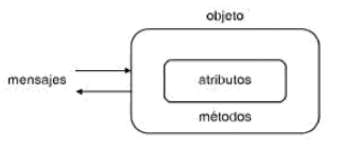
\includegraphics[width=0.35\textwidth]{images/Capture0001.PNG}
        }
        \caption{Diseño de una clase de objetos.}
        {{\footnotesize Fuente: Programación Orientada a Objetos con C++.}}
        \label{figdisenioclases}
    \end{figure}

    \subsection{Ajedrez}
    
    La principal leyenda del origen de este milenario juego comienza con un rey de la India llamado Belkib, que estando aburrido ofreció una recompensa a cambio de distracción, el sabio Sissa le propuso el ajedrez, a cambio del juego le pidió un grano de trigo por el primer recuadro del tablero, por el segundo el doble y así doblando la cantidad, al rey le pareció modesta la cantidad pero luego se dio cuenta que habría que depositar más de nueve billones de granos de trigo \citep{origenajedrez}.
    \begin{figure}[ht]
        \centering{
            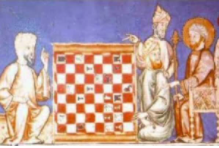
\includegraphics[width=0.2\textwidth]{images/Capture0002.PNG}
        }
        \caption{Origen del ajedrez.}
        {{\footnotesize Fuente: CurioSfera.com}}
        \label{figdajedrezold}
    \end{figure}
    Nosotros conocemos ahora un tablero cuadriculado con casillas negras y blancas, con variedad de fichas diferentes con diversa posibilidad de movimientos, en un comienzo se tenía el consejero o ministro que era el compañero del rey, este se convirtió en la Edad Media, en la figura de la reina, al principio también era una pieza más débil de la misma forma del rey, pero en siglo XV se convirtió en la figura más importante del ajedrez. Una curiosidad importante sobre la historia del ajedrez es que los reyes de algunos países les gustaba jugar al ajedrez humano.
    \newline
    \newline
    \tab[0.55cm] Existen diversos detalles básicos, encontramos 32 piezas en el tablero de 64 casilleros, cada jugador tiene 6 tipos distintos de piezas: 8 peones, 2 torres, 2 caballos, 2 alfiles, una reina y un rey.
    \newline
    \newline
    \tab[0.55cm] El peon es la pieza de menor valor en el ajedrez, cada jugador tiene 8 peones, tienen menos opciones de movimiento, en la primera jugada pueden avanzar dos casillas. En los demás casos puede avanzar solo una casilla hacia adelante. La excepción es cuando se captura una pieza enemiga, en este caso se mueve a una casilla en forma diagonal, siempre hacia adelante, podemos observar esto en la figura \ref{fig:peonM}. La torre es una pieza pesada en Ajedrez, al empezar la partida cada jugador tiene dos piezas de estas. El movimiento que realizan es el más fácil de todos. Las torres se mueven para adelante, atrás, izquierda y derecha, solo una dirección a la vez, observamos el movimiento en la figura  \ref{fig:torreM}.
    
    \begin{figure}[h!]
    \centering
    \begin{subfigure}[b]{0.45\linewidth}
    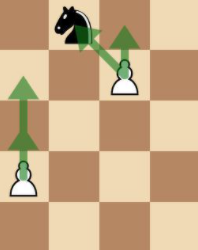
\includegraphics[width=\linewidth]{images/Capturep01.PNG}
    \caption{Movimientos del peón}
    \label{fig:peonM}
    \end{subfigure}
    \begin{subfigure}[b]{0.455\linewidth}
    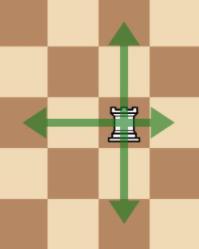
\includegraphics[width=\linewidth]{images/Capturep02.PNG}
    \caption{Movimiento de la torre}
    \label{fig:torreM}
    \end{subfigure}
    \caption{Movimientos de las piezas - Parte 1}
    {{\footnotesize Fuente: ichess.es}}
    \label{fig:westminster}
    \end{figure}
    
    \begin{figure}[h!]
    \centering
    \begin{subfigure}[b]{0.45\linewidth}
    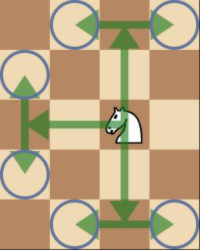
\includegraphics[width=\linewidth]{images/Capturep03.PNG}
    \caption{Movimientos del caballo}
    \label{fig:caballoM}
    \end{subfigure}
    \begin{subfigure}[b]{0.445\linewidth}
    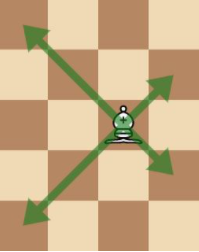
\includegraphics[width=\linewidth]{images/Capturep04.PNG}
    \caption{Movimientos del alfil}
    \label{fig:alfilM}
    \end{subfigure}
    \caption{Movimientos de las piezas - Parte 2}
    {{\footnotesize Fuente: ichess.es}}
    \label{fig:westminster}
    \end{figure}
    
    El caballo es una de las piezas menores, al inicio de la partida tenemos dos de estas piezas. Su movimiento es muy particular, puede ser muy confuso para los principiantes en el juego y es la única pieza que puede saltar sobre las otras. El caballo se mueve en forma de L, dando solo 3 pasos, el movimiento se puede observar en la figura \ref{fig:caballoM}. El alfil también es considerada como otra pieza menor en el tablero, también se cuentan con dos piezas. Su movimiento es en diagonal, uno de los alfiles por las casillas claras y el otro por las casillas oscuras, sus movimientos se observan en la figura \ref{fig:alfilM}.
    \newline
    \newline
    \tab[0.55cm] La reina es la pieza más poderosa en una partida de ajedrez y más importante luego del rey. Cada jugador tiene una sola dama, la dama puede moverse en cualquier dirección y tantas casillas como quiera, lo único que no puede hacer es saltar sobre las otras piezas, el movimiento se observa en la figura \ref{fig:reinaM}. Finalmente tenemos la pieza más importante de cualquier partida de ajedrez, el objetivo principal de la partida es dar jaque mate al rey opuesto, por ello el rey no puede ser capturado, sus movimientos son bastante limitados, una casilla en cualquier dirección, pero solo si no se encuentra amenazado en la casilla que se quiere mover, observamos mejor el movimiento en la figura \ref{fig:reyM}, el rey también puede realizar el movimiento llamado enroque, donde se protege con la ayuda de una torre.
 \newline
    \newline
    \tab[0.55cm] Entonces conociendo que en el ajedrez podemos considerar cada una de las piezas del tablero como distintos objetos, podemos realizar la programación de este juego con la técnica de programación orientada a objetos, aplicar conceptos también de polimorfismo, como sabemos cada una de las fichas tienen distintas imágenes y movimientos, pero también es una característica que comparten todas, todas tienen una imagen que las representa y también todas tienen movimientos que las representan. Esto se explicará más a detalle en en apartado de Técnicas de Programación Orientada a Objetos implementadas.
    
    \begin{figure}[h!]
    \centering
    \begin{subfigure}[b]{0.45\linewidth}
    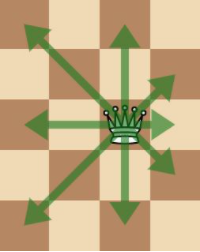
\includegraphics[width=\linewidth]{images/Capturep05.PNG}
    \caption{Movimientos de la reina}
    \label{fig:reinaM}
    \end{subfigure}
    \begin{subfigure}[b]{0.45\linewidth}
    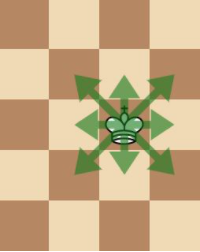
\includegraphics[width=\linewidth]{images/Capturep06.PNG}
    \caption{Movimientos del rey}
    \label{fig:reyM}
    \end{subfigure}
    \caption{Movimientos de las piezas - Parte 3}
    {{\footnotesize Fuente: ichess.es}}
    \label{fig:westminster}
    \end{figure}

\section{Materiales}

    \subsection{C++}
    Para el desarrollo del proyecto utilizamos la versión 4 de C++, como sabemos los lenguajes de programación están en constante evolución, la primera versión de C++ se lanzó en 1985, en la década de los 90 este lenguaje fue considera estándar y en 1998 ISO lo ratificó dando lugar al primer dialecto de C++ que se conoció como C++98. En los cambios que se tuvieron con C++11 fueron \citep{c11}:
    \begin{itemize}
        \item Auto: Introduce la inferencia de tipos con la palabra clave \textit{auto}, donde el compilador infiere el tipo de una variable en el punto de la declaración.
        \item \textit{nullptr}: Anteriormente se tenía la constante 0 como un doble papel de entero constante y constante de puntero nulo. En esta versión se corrige eso con la nueva palabra clave.
        \item \textit{shared\_ptr}: El puntero inteligente no fue un concepto nuevo, fue implementado en algunas bibliotecas, pero se estandarizó ya no es necesario utilizar una biblioteca externa.
        \item  C++11 introduce las palabras clave de la clase \textit{enum}. Donde ya no exportan sus enumeradores en el ámbito circundante. Ahora se pueden heredar de una numeración.
        \item \textit{Loops} basados en rango: Se aumentó la instrucción for para respaldar el paradigma \textit{foreach} de iterar sobre colecciones, para realizar un código más simple y limpio.
        \item \textit{Lambda}: C++11 brinda la capacidad de crear funciones anónimas, que son conocidas como \textit{lambda}.
    \end{itemize}
    
        \begin{figure}[ht]
        \centering{
            
\includegraphics[width=0.2\textwidth]{images/c++11.PNG}
        }
        \caption{C++11.}
%        {{\footnotesize Fuente: CurioSfera.com}}
        \label{figiconqt}
    \end{figure}

    \subsection{Qt}
    
    Qt es un framework orientado a objetos para desarrollar programas que necesiten una interfaz gráfica de usuario, esta desarrollada como un software libre y de código abierto \citep{qtframework} \citep{qt}.
    \newline
    \newline
    \tab[0.55cm] Fue desarrollado inicialmente por Haavard Nord y Eirik Chambe-Eng, ambos con maestrías en ciencias de la computación. El kit de herramientas se llamó QT ya que la letra Q lucía atractiva en la fuente Emacs y T se inspiró en Xt, el kit de herramientas X, X Tool kit.
    \newline
    \newline
    \tab[0.55cm] Qt Creator es un IDE (entorno de desarrollo integrado) multiplataforma que se adecua a las necesidades de los desarrolladores. Se puede usar tanto en Windows, MacOs o Linux.
    \newline
    \tab[0.55cm] Posee algunas características como:
    \begin{itemize}
        \item Editor de código con soporte para C++, .NET, Python, Ada, PHP, etc.
        \item Trae un GUI integrado.
        \item Nos proporciona una navegación rápida en el código.
        \item Resaltado de la sintaxis y autocompletado de código.
        \item Ayuda sensitiva al contexto.
    \end{itemize}
    \newline
    \newline
    \tab[0.55cm] Qt Creator también cuenta con algunas herramientas extras aparte del editor de código como:
    \begin{itemize}
        \item qmake: Es el sistema de compilación estándar de Qt, se encuentra integrado en Qt Creator, pero también es compatible con otros sistemas de compilación como cmake.
        \item Qt Designer: Es el programa nativo para diseñar y desaroolar interfaces gráficas de usuario con ayuda de Qt Widgets. Este editor permite colocar y ajustar widgets como se desee.
        \item Qt Assistant: Con Qt Assistant brinda un acceso rápido a documentación oficial.
    \end{itemize}
    \newline
    \newline
    \tab[0.55cm] Sobre esta herramienta podemos decir que permite desarrollar aplicaciones con el lenguaje C++ para escritorio y con interfaces de usuario (UI) personalizables, nos permite trabajar con un sistema de compilación que nos facilita trabajar con los diversos archivos que se necesitan en el desarrollo de software. 

    \begin{figure}[ht]
        \centering{
            
\includegraphics[width=0.2\textwidth]{images/descarga (1).png}
        }
        \caption{Qt logo.}
%        {{\footnotesize Fuente: CurioSfera.com}}
        \label{figiconqt}
    \end{figure}
    
    \subsection{Git}
    Git es un sistema de control de versiones de código abierto que fue iniciado por Linus Torvalds. Es similar a otros sistemas de control de versiones como: Subversión, CVS, Mercurial. Esto significa que cuando los desarrolles crean algo, se realizan cambios constantes en el código, se van lanzando nuevas versiones hasta y después del primer lanzamiento oficial (no beta) \citep{github}.
    \newline
    \newline
    \tab[0.55cm] Los sistemas de control de versiones mantienen las revisiones en orden, permite la colaboración de los desarrolladores, pueden descargar versiones nuevas del software, realizar cambios y cargar la versión más reciente. Todos los desarrolladores pueden ver cambios, descargarlos y contribuir.
    \newline
    \newline
    \tab[0.55cm] Git es el sistema de control de versiones preferido de la mayoría de desarrolladores, tiene ventajas sobre otros sistemas, como almacenar cambios de archivos de manera más eficiente y también garantiza la integridad de los archivos.
    \newline
    \newline
    \tab[0.55cm] Como sabemos Git es una herramienta de línea de comandos, GtHub es donde los desarrolladores almacenan sus proyectos y se conectan con personas de ideas afines.
    \newline
    \newline
    \tab[0.55cm] Tenemos lo que es un repositorio, es una ubicación donde se almacenan todos los archivos de un proyecto. Cada proyecto tiene su propio repositorio y se permite acceder al mismo con una URL única.
    \begin{figure}[ht]
        \centering{
            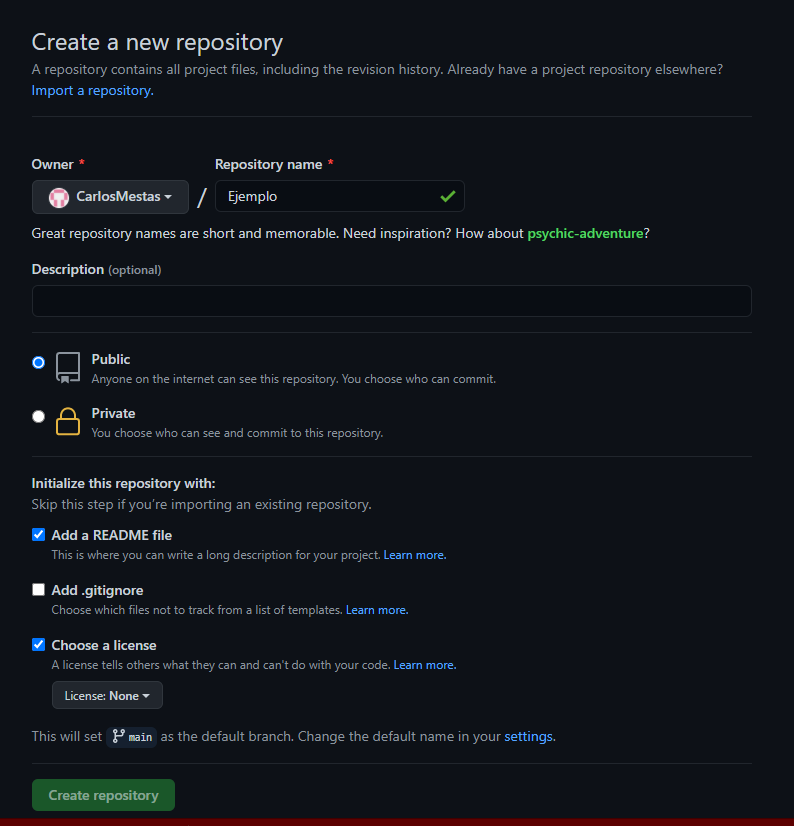
\includegraphics[width=0.5\textwidth]{images/Capture00003.PNG}
        }
        \caption{Creación de un repositorio en GitHub.}
%        {{\footnotesize Fuente: CurioSfera.com}}
        \label{figiconqt}
    \end{figure}
    \newline
    \tab[0.55cm] Una de las características principales es que GitHub no es solo para programadores, a pesar de que se mencionó que los desarrolladores la usan para controlar los diversos archivos de un proyecto, se pueden usar GitHub para cualquier tipo de archivo. Por ejemplo un equipo de trabajo que realiza cambios en un documento de Word, puede usar GitHub para controlar las versiones de los documentos, no es una práctica muy común, pero es algo que se puede tomar en cuenta.
    
    \subsection{Others}
    
        \subsubsection{Google Meet}
        Es una herramienta que nos permitió realizar reuniones grupales, se puede usar tanto en navegadores web y dispositivos móviles, para acceder a esta herramienta solo necesitamos acceder a la página \textcolor{blue}{
        \href{meet.google.com}{meet.google.com}} o también poder descargar la aplicación para Android e iOS. Se crean códigos de reunión únicos para cada videollamada. Es un método seguro, solo los usuarios que disponen del código tendrán acceso a las reuniones. También se pueden programar estas reuniones a través de Google Calendar \citep{meet}.
        
        \begin{figure}[ht]
            \centering{
                
\includegraphics[width=0.5\textwidth]{images/google meet.png}
            }
            \caption{Google meet.}
    %        {{\footnotesize Fuente: CurioSfera.com}}
            \label{figiconqt}
        \end{figure}
        
        \subsubsection{Discord} 
        Es una plataforma que permite crear servidores de chat con el cual los usuarios pueden reunirse para hablar en comunidades. Para nuestro trabajo nos permitió la comunicación un poco menos formal a comparación de Google Meet para las reuniones grupales, compartir código, etc., la creación de un servidor para la comunicación es sencilla y para las salas tanto de texto como de voz son sencillas de usar, luego se crean códigos de invitación para los usuarios participantes.
            
         \begin{figure}[ht]
            \centering{
                
\includegraphics[width=0.15\textwidth]{images/discord.png}
            }
            \caption{Discord.}
    %        {{\footnotesize Fuente: CurioSfera.com}}
            \label{figimeet}
        \end{figure}   
        

\section{Métodos}

    \subsection{Diagrama de clases}
    
        Sabemos que un diagrama de clases en Lenguaje Unificado de Modelado (UML) es un tipo de diagrama de estructura estática que describe la estructura de un sistema, mostrando las clases del sistema, atributos, métodos y relaciones entre los objetos.
        \newline
        \newline
        \tab[0.55cm] Permite organizar el sistema que nuestro equipo comenzó a desarrollar, ayuda a la implementación del sistema y ver esquemas lógicos de la estructura de datos.
        \newline
        \newline
        \tab[0.55cm] Podemos observar el desarrollo del diagrama desarrollado en la figura, \ref{fig:diagramaclases}, donde podemos observar que cada una de las piezas del ajedrez como los peones, caballos, alfiles, torres, dama y rey heredan de la clase Pieza, el constructor que utilizan es el mismo básicamente, pero se van a manejar diferencias con respecto a la elección de las imágenes para cada pieza, como por ejemplo en el caso del caballo, se necesita información de la imagen, y esta también varía de acuerdo al color de la ficha, la imagen que estamos cargando depende del equipo al cual pertenece la ficha y también con el método de movimientos podemos agregar los diversos movimientos que pueden realizar cada una de las fichas. 
        \newline
        \newline
        \tab[0.55cm] La clase casilla tiene métodos que nos permiten conocer el evento del \textit{mouse} al momento que se presiona esta pieza, también nos brinda información de la casilla actual a la que pertenece, uno de sus atributos también es la casilla que es a donde pertenece, por lo cual también tiene un método \textit{get} que permite obtener información del casillero, la clase Casilla tiene un atributo  \textit{bool} que indica si tiene una pieza o no e información que va a pertenecer a la pieza, como posición y el color también de la pieza, tenemos luego nuestra clase Tablero que es la clase que esta relacionada a la cantidad de casillas que contiene un tablero de ajedrez, en este caso tenemos 64 casilleros que pertenecen a un tablero. 
        \newline
        \newline
        \tab[0.55cm] Tenemos también otras clases, como la clase \textit{Time} que nos a permitir trabajar con cronómetros, como se conoce en el juego de ajedrez cada jugador tiene un límite de tiempo para poder realizar sus movimientos, entonces se utilizarán dos cronómetros para medir el tiempo de cada jugador mientras va jugando y finalmente tenemos la clase \textit{Log}, esta clase nos permite realizar una impresión en pantalla de información sobre los movimientos, en este caso en un tablero se conoce las posiciones de cada ficha, mediante una matriz de números con letras, entonces con la clase \textit{Log} podremos obtener información de las jugadas que realiza el jugador con las diversas piezas.
        
        
    \subsection{Técnicas de POO implementadas}

        \subsubsection{Herencia}
        La herencia es uno de los conceptos básicos de la programación orientada a objetos, ya que puede reutilizar variables y funciones definidas en otras clases. Para hablar de herencia, se deben introducir los conceptos de clases base y derivadas. La clase que pretende heredar sus propiedades (variables) y funciones (métodos) a otras clases se llama clase base. Por otro lado, las clases derivadas se denominan clases que se implementan reutilizando atributos y funciones heredadas de una (o más) clases base. La herencia ayuda a mejorar la escalabilidad de la aplicación hasta cierto punto, porque cuando las variables o métodos heredados deben ser modificados o eliminados en todas las clases derivadas, no es necesario tratarlos por separado en cada clase, sino directamente en la aplicación. Completado en la clase del programa. Las clases base y las clases derivadas solo heredan y se actualizan de estos miembros.
        \newline
        \newline
        \newline
        \tab[0.55cm] En C ++, la herencia se expresa en la implementación de una clase mediante el operador de dos puntos, seguido del tipo de herencia (lo presentaremos más adelante) y el nombre de la clase base de la que se heredará. Vale la pena señalar que el tipo de herencia predeterminado en C ++ es herencia privada sin especificar el campo explícitamente. Esta es la implementación más simple del concepto de herencia en C ++:
        \subsubsection{Polimorfismo}
        Esta técnica de programación orientada a objetos nos a permitido trabajar con mayor facilidad al momento de trabajar con las distintas clases que tenemos, se pueden observar en la figura \ref{fig:diagramaclases}, podemos escribir los objetos en forma genérica, como objetos de clase base para un conjunto de clases existentes, mediante una jerarquía, en este caso tenemos una clase general la clase Pieza, y las demás clases que están bajo mediante jerarquía que son cada una de las piezas del ajedrez, en este caso: Peon, Caballo, Alfil, Torre, Dama y Rey. 
        \newline
        \newline
        \tab[0.55cm] Como sabemos entonces las distintas piezas son derivadas de la clase Pieza, como sabemos todas tienen características similares en este caso un método donde se agregue la imagen a cada una de las piezas y también agregar los movimientos, en este caso todos cuentan con distintas imágenes y movimientos, pero en general realizan las mismas acciones. Al momento de llamar a la función de setImagen que pertenece a la clase base Pieza y de esa forma el programa determina en tiempo de ejecución que función de setImagen de la clase derivada se va a utilizar. Este comportamiento se consigue cuando declaramos en la clase base la función como virtual y en cada una de las clases derivadas se van sobreponiendo para colocar en este caso la imagen adecuada o en caso contrario también se van a colocar los movimientos que pueden realizar cada una de las piezas del juego de ajedrez.
        \newline
        \newline
        \tab[0.55cm] C++ permite utilizar el polimorfismo, para que en un programa se tenga poliformismo tenemos que tener \citep{polimorfismo}:
        \begin{itemize}
            \item Tener una jerarquía de clases, donde las operaciones importantes, funciones, están declaras en métodos virtuales.
            \item Manipular los objetos a través de punteros.
        \end{itemize}
        \newline
        \newline
        \newline
        \tab[0.55cm] Un ejemplo claro de polimorfismo se puede observar en la figura \ref{figifigur}, donde tenemos en este caso la clase abstracta Figura que es nuestra clase base y las clases derivadas Circulo y Cuadrado, la clase base tiene métodos virtuales, que cada una de las clases derivadas implementa de manera distinta, ambas tienen lo que es un perímetro y área pero la forma de calcularlos es distinta.
            
         \begin{figure}[ht]
            \centering{
                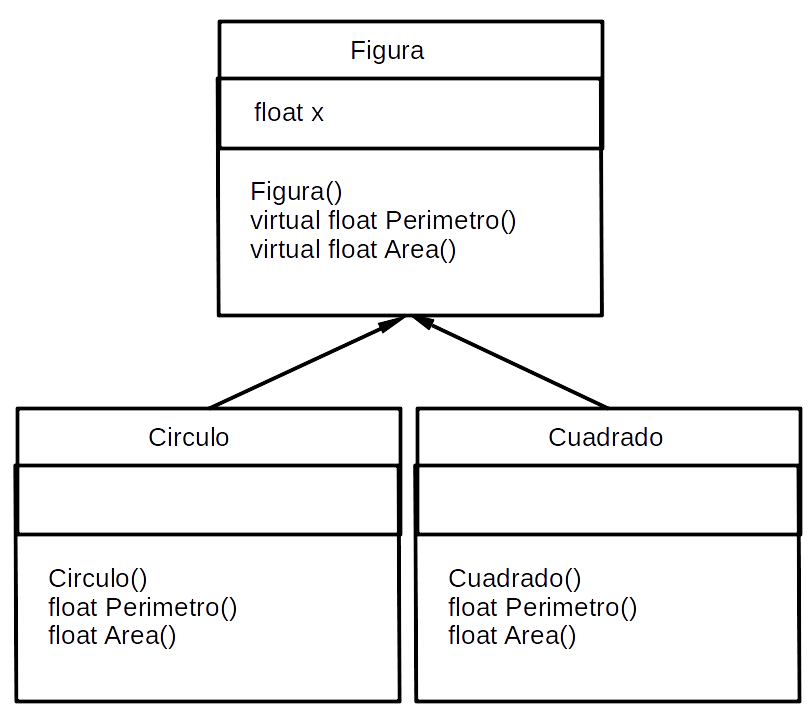
\includegraphics[width=0.35\textwidth]{images/diagrama_de_objetos2.png}
            }
            \caption{Ejemplo polimorfismo.}
           {{\footnotesize Fuente: LabSCN}}
            \label{figifigur}
        \end{figure}   
     
        
\section{Guía}
Tenemos la primera interfaz donde podemos seleccionar el modo en el cual deseamos jugar, figura \ref{interfazInicio}, podemos seleccionar con o sin cronometro, en este caso si seleccionamos con cronómetro podemos observar en la figura \ref{InterfazCompleta}, en el lado izquierdo se puede observar el cronómetro que pertenece la jugador de las piezas blancas y también los movimientos que esta realizando, observamos eso en las figuras \ref{figcronometro y log} y \ref{Ubicacion del cronometro y log}, para los movimientos de las diversas piezas estas ya están programadas, entonces al momento de seleccionar una pieza nos mostrará los posibles movimientos, unos ejemplos de esta funcionalidad se encuentra en las figuras \ref{posibles movimientoscaballonegro} y \ref{posibles movimientosdamanegra} y finalmente tenemos el jaque, cuando el rey del oponente esta amenazado por una de nuestras piezas entonces se pintará la casilla de color azul, figura \ref{Jaque al rey}.


\section{Conclusiones}

    \newline
    \newline
    \tab[0.55cm]Logramos aprender en el curso de Tecnología de Objetos conocimientos sobre la programación orientada a objetos y cómo podemos llegar a aplicarla a ejemplos reales, en este caso más específico en el juego de ajedrez.
    \newline
    \newline
    \tab[0.55cm]La primera dificultad que tuvimos la encontramos al intentar gráficar el tablero, previamente teníamos un tablero que podía redimensionarse a cualquier escala, sin embargo esto nos dio la dificultad de no poder tener la ubicación precisa de las piezas, originando que nos replanteemos usar un tamaño exacto.
    \newline
    \newline
    \tab[0.55cm]El segundo problema que se nos presento fue el \textit{drag and drop}, se intento usar este, sin embargo había en ciertos momentos que la pieza se iba a una ubicación que no esperábamos, no logramos usar este método restringiendo sus movimientos de la manera que esperamos. Se uso \textit{click events} para realizar el movimiento de la pieza, asemejándose a un \textit{drag and drop}.
    \newline
    \newline    
    \tab[0.55cm]El tercer problema que tuvimos fue implementar todos los movimientos que se pueden hacer en el ajedrez, hay ciertos movimientos los cuales no se pudieron implementar en la totalidad, como es el caso del enroque, la promoción y cuando se consideraría un jacke y jacke mate.
    
    
    
La primera dificultad que se encontró, fue con el drag and drop, puesto que 

\AtNextBibliography{\small}\printbibliography

\section{Anexos}

\clearpage
\newpage

\begin{figure*}
  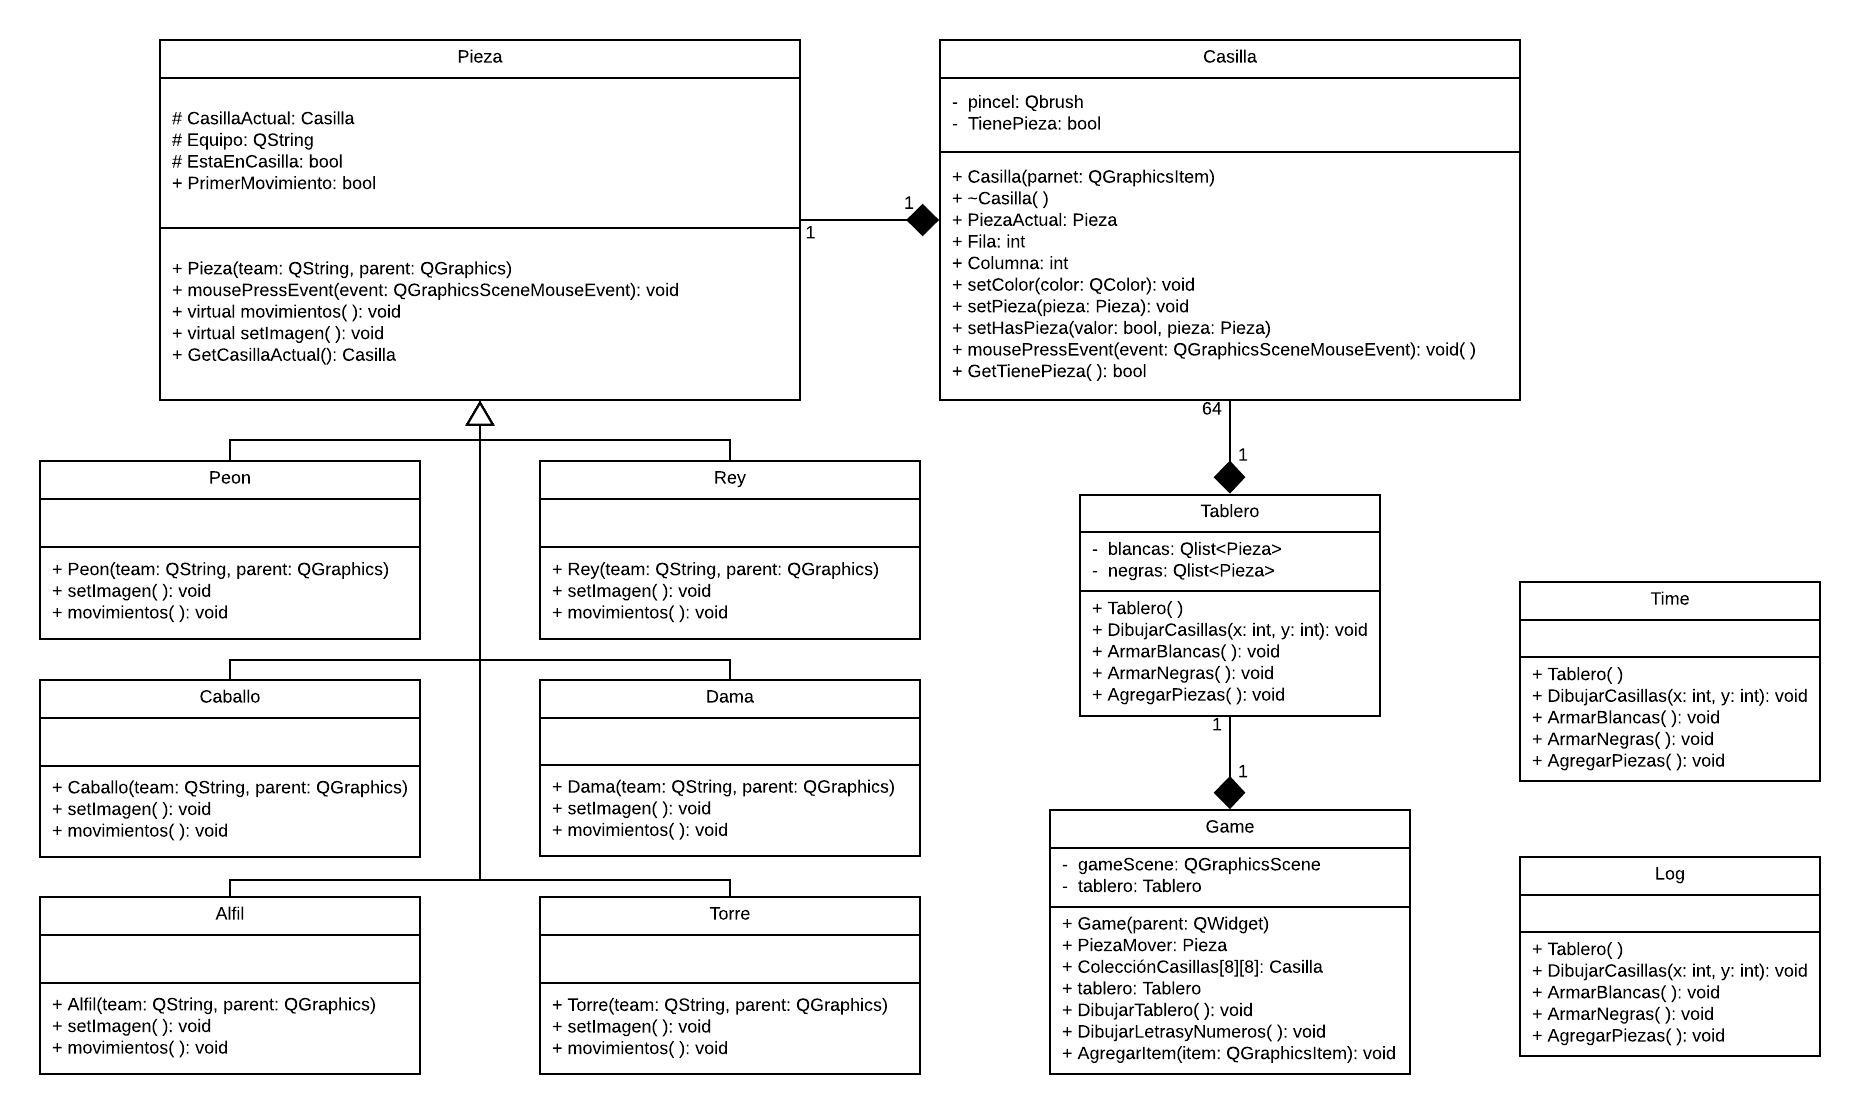
\includegraphics[width=1\textwidth]{images/cc.jpeg}
  \caption{Diagrama de clases.}
  \label{fig:diagramaclases}

\end{figure*}

\begin{figure}[ht]
        \centering{
            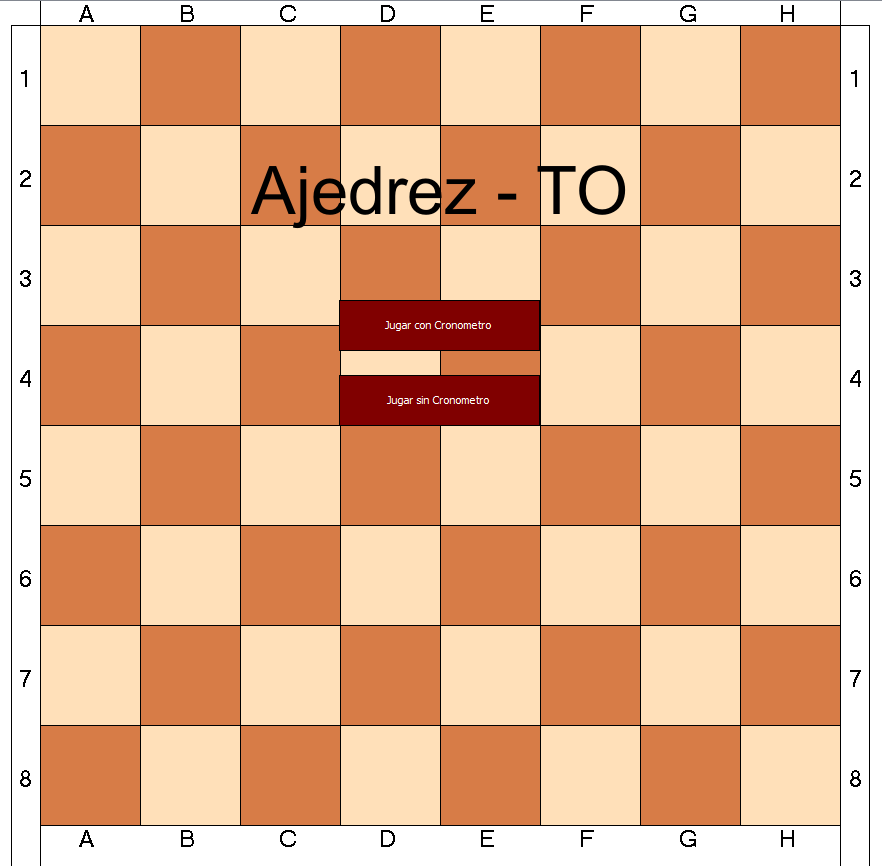
\includegraphics[width=0.5\textwidth]{images/Tablero.png}
        }
        \caption{Interfaz inicio}
%        {{\footnotesize Fuente: CurioSfera.com}}
        \label{interfazInicio}
    \end{figure}
    
    \begin{figure}[ht]
        \centering{
            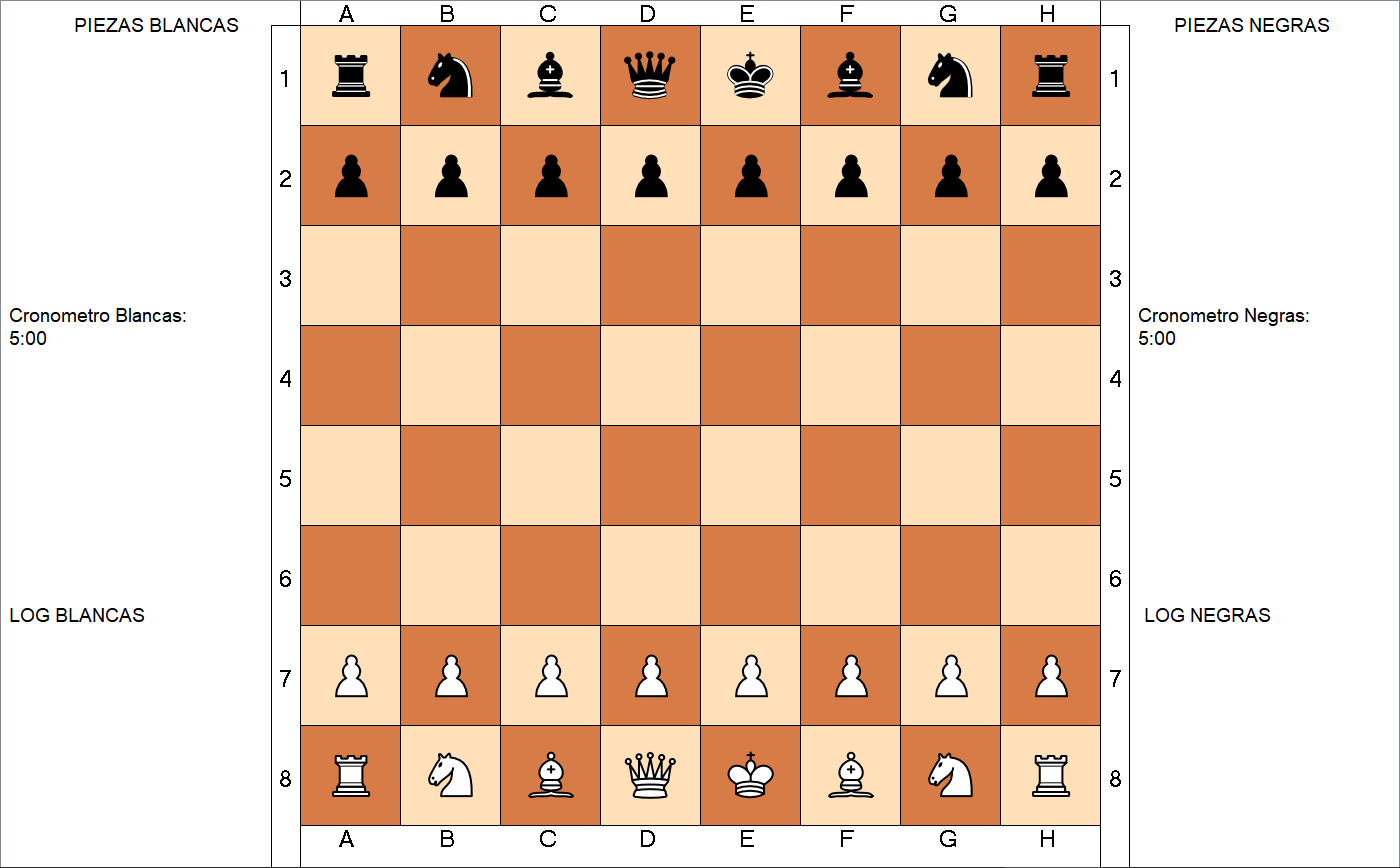
\includegraphics[width=0.5\textwidth]{images/Tablero2.png}
        }
        \caption{Interfaz con cronómetro.}
%        {{\footnotesize Fuente: CurioSfera.com}}
        \label{InterfazCompleta}
    \end{figure}
    
    \newline
    
    \begin{figure}[ht]
        \centering{
            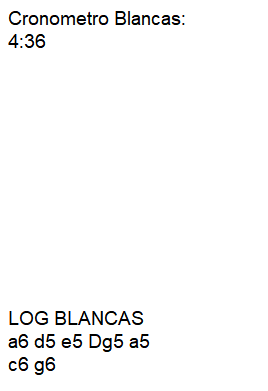
\includegraphics[width=0.5\textwidth]{images/Tablero3.png}
        }
        \caption{Cronómetro y log para el jugador de fichas blancas.}
%        {{\footnotesize Fuente: CurioSfera.com}}
        \label{figcronometro y log}
    \end{figure}
    
    \begin{figure}[ht]
        \centering{
            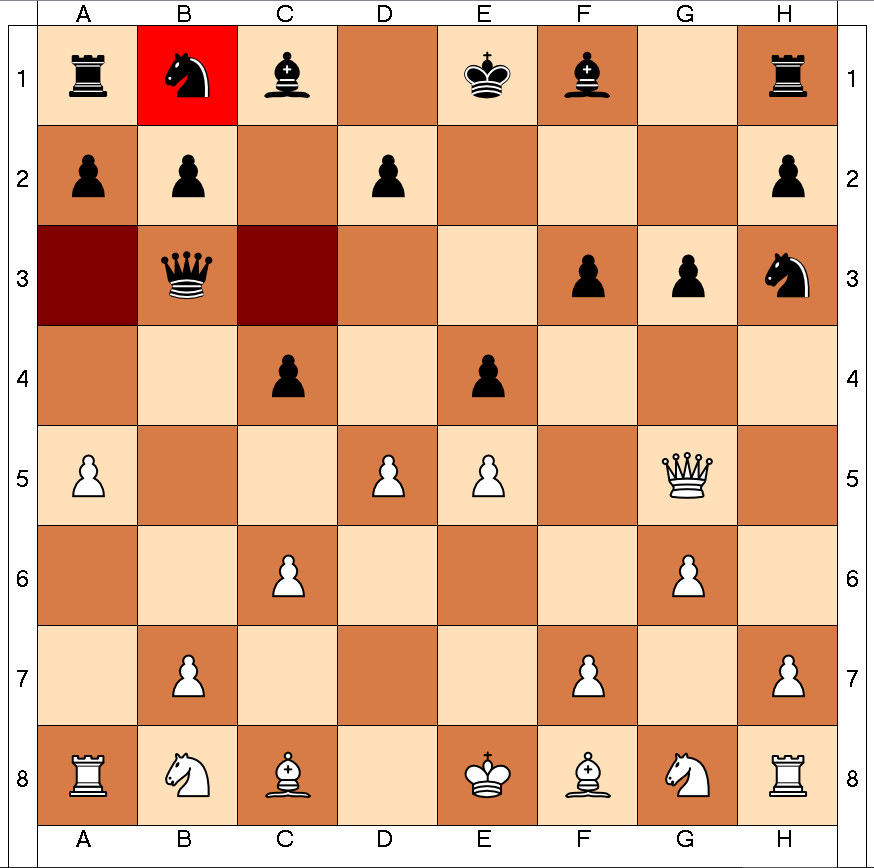
\includegraphics[width=0.5\textwidth]{images/Tablero4.png}
        }
        \caption{Posibles movimientos del caballo negro.}
%        {{\footnotesize Fuente: CurioSfera.com}}
        \label{posibles movimientoscaballonegro}
    \end{figure}
    
    \begin{figure}[ht]
        \centering{
            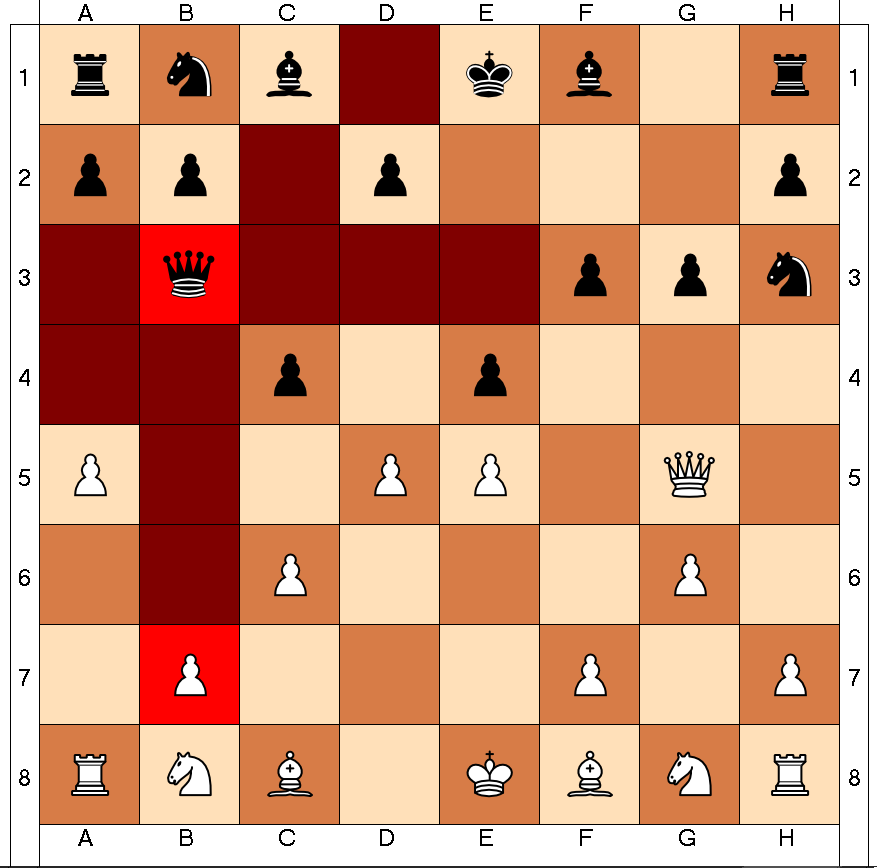
\includegraphics[width=0.5\textwidth]{images/Tablero5.png}
        }
        \caption{Posibles movimientos de la dama negra.}
%        {{\footnotesize Fuente: CurioSfera.com}}
        \label{posibles movimientosdamanegra}
    \end{figure}
    
    \begin{figure}[ht]
        \centering{
            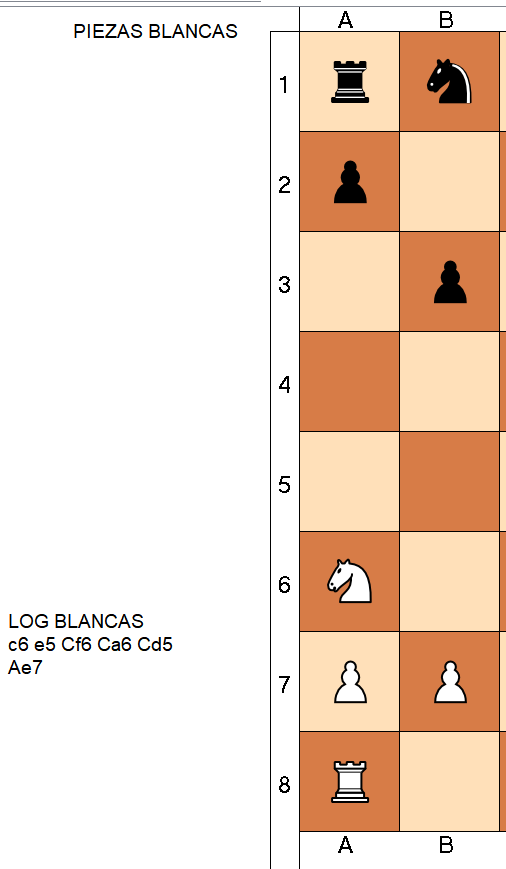
\includegraphics[width=0.5\textwidth]{images/Tablero6.png}
        }
        \caption{Ubicación del cronómetro y el log de las fichas blancas.}
%        {{\footnotesize Fuente: CurioSfera.com}}
        \label{Ubicacion del cronometro y log}
    \end{figure}
    
    \begin{figure}[ht]
        \centering{
            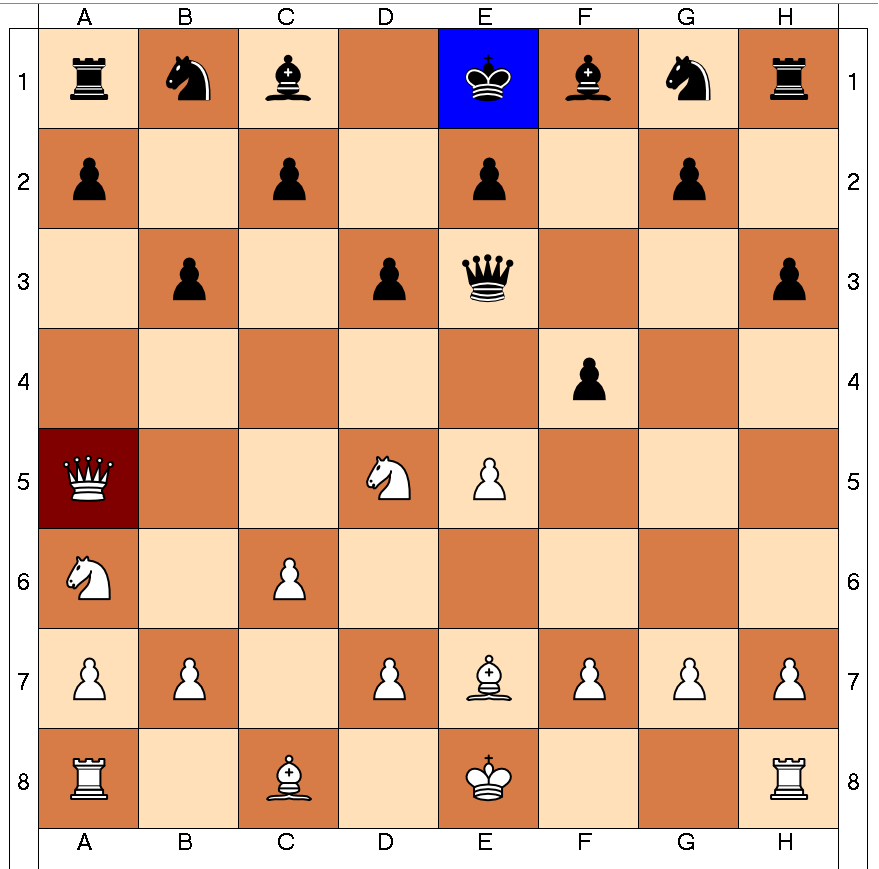
\includegraphics[width=0.5\textwidth]{images/Tablero7.png}
        }
        \caption{Vista cuando ocurre un jaque al rey.}
%        {{\footnotesize Fuente: CurioSfera.com}}
        \label{Jaque al rey}
    \end{figure}
    

\end{document}
